%!TEX program = xelatex
% 完整编译: xelatex -> bibtex -> xelatex -> xelatex
\documentclass[lang=cn,11pt,a4paper]{elegantpaper}
\usepackage{listings}
\usepackage{color}
\usepackage[ruled]{algorithm2e}
\usepackage{graphicx}

\usepackage{subfigure}
\usepackage{multicol}  
\usepackage{multirow}

\definecolor{darkblue}{rgb}{.0, .0,.6}
\definecolor{red}{rgb}{1.0,.0,.0}
\definecolor{green}{rgb}{.25,.8,.35}
\definecolor{pinkgrey}{rgb}{.95,.8,.8}
\definecolor{mist}{rgb}{.8,.8,.95}

\lstset{
    basicstyle          =   \sffamily,          % 基本代码风格
    keywordstyle        =   \bfseries,          % 关键字风格
    commentstyle        =   \rmfamily\itshape,  % 注释的风格,斜体
    stringstyle         =   \ttfamily,  % 字符串风格
    flexiblecolumns,                % 别问为什么,加上这个
    numbers             =   left,   % 行号的位置在左边
    showspaces          =   false,  % 是否显示空格,显示了有点乱,所以不现实了
    numberstyle         =   \zihao{-5}\ttfamily,    % 行号的样式,小五号,tt等宽字体
    showstringspaces    =   false,
    captionpos          =   t,      % 这段代码的名字所呈现的位置,t指的是top上面
    frame               =   lrtb,   % 显示边框
}

\lstdefinestyle{Python}{
    language        =   Python, % 语言选Python
    basicstyle      =   \zihao{-5}\ttfamily,
    numberstyle     =   \zihao{-5}\ttfamily,
    keywordstyle    =   \color{blue},
    keywordstyle    =   [2] \color{teal},
    stringstyle     =   \color{magenta},
    commentstyle    =   \color{red}\ttfamily,
    breaklines      =   true,   % 自动换行,建议不要写太长的行
    columns         =   fixed,  % 如果不加这一句,字间距就不固定,很丑,必须加
    basewidth       =   0.5em,
}

\newcommand{\Blue}[1]{\textcolor[rgb]{0,0,0.803}{#1}}
\newcommand{\red}[1]{\textcolor[rgb]{1,0,0}{#1}}

\usepackage{array}
\usepackage{amsfonts}
\newcommand{\f}[0]{\mathcal{F}}
\newcommand{\A}[0]{\mathcal{A}}
\newcommand{\p}[0]{\mathbb{P}}
\newcommand{\cc}[0]{\mathcal{C}}
\newcommand{\R}[0]{\mathbb{R}}
\newcommand{\D}[0]{\mathcal{D}}
\newcommand{\V}[0]{\mathcal{V}}
\newcommand{\M}[0]{\mathcal{M}}
\newcommand{\T}[0]{\mathcal{T}}
\newcommand{\s}[2]{\sum_{#1}^{#2}}



\title{实用统计软件项目报告}
\author{晏若儒 \\ PB17081535 \and 骆霄龙 \\ PB18151853}
\institute{论文: A convex formulation for high-dimensional sparse
sliced inverse regression}

\date{\zhtoday}

\begin{document}

\maketitle
\tableofcontents
\newpage

\begin{abstract}
本文主要是使用切片逆回归方法处理高维度情形下的稀疏回归问题,通过结合交替方向乘子算法来迭代求解中心降维子空间。对估计误差的上界给出了理论证明并进行了模拟实验。 
基于我们选择的文章,我们实现了文中的切片逆回归 结合 交替方向乘子的算法,并复现了文中的实验,取得了比较一致的结果。同时我们将文中的算法在不同模型下与Lasso,Ridge,ElasticNet 这三个方法进行了比较,来考察不同方法的优劣性。

\href{代码链接}{(代码链接:https://github.com/lxl213)}
\keywords{凸优化问题,降维,切片逆回归,交替方向乘子算法,R语言,不同模型下优化方法比较}
\end{abstract}


\section{文章内容概述}


\subsection{问题背景}
考虑在高维情形下的回归问题(样本数量n 小于 变量数目d):  
$y = f(x)$,当变量数目d很大时,我们希望能对变量进行降维,找出显著的变量并尽可能少的损失信息。我们考虑在满足以下条件下的降维问题: 

\begin{equation}
    y \Perp x \mid\left(\beta_{1}^{\mathrm{T}} x, \ldots, \beta_{K}^{\mathrm{T}} x\right)
\end{equation}

其中 $ K< min (n,d), \beta_1, \cdots , \beta_K \in \R^d, \Perp \text{表示独立} $ .所以方程(1)表示y能够被x的K个线性组合所决定。 我们称$\beta_1, \cdots , \beta_K$为充分降维方向(sufficient dimension
reduction directions),$ \V  = span{\beta_1, \cdots , \beta_K}$,由于$ \V$不唯一,我们称 $ \V_{y|x} = \cap \V$为中心降维子空间(central dimension reduction subspaces)。 这篇文章中 使用 基于切片逆回归法( sliced inverse regression)的改进方法来 估计d>n时的中心降维子空间 $ \V_{y|x}$。

\subsection{主要工作}

\begin{itemize}
    \item 对论文理论部分进行了较为完善的总结,给出了文章提出方法的主要思路和具体解法
    \item 对文章算法进行了复现,并进行实验取得了与文章较为一致的成果
    \item 实现了在文章中三个模型下的其他回归算法,并做图与文章算法进行比较与分析
    
\end{itemize}

\subsection{主要理论}
考虑上述回归模型的一般形式:
\begin{equation}
y=f\left(\beta_{1}^{\mathrm{T}} x, \ldots, \beta_{K}^{\mathrm{T}} x, \epsilon\right)
\end{equation}
在使用切片逆回归法(下面简称SIR)时一个需要一个线性条件,对 $ \forall a \in \R^d$:
\begin{equation}
    E\left(a^{\mathrm{T}} x \mid \beta_{1}^{\mathrm{T}} x, \ldots, \beta_{K}^{\mathrm{T}} x\right)=b_{0}+b_{1} \beta_{1}^{\mathrm{T}} x+\cdots+b_{K} \beta_{K}^{\mathrm{T}} x
\end{equation}
在线性条件(3)下, 由(Li, 1991\cite{1991_paper}, Theorem 3.1 ).问题转化为寻找$ V \in \R^{d \times K}$使得:

\begin{equation}
    \hat{\Sigma}_{E(x \mid y)} V=\hat{\Sigma}_{x} V \Lambda
\end{equation}
其中$\hat{\Sigma}_{E(x \mid y)} \text{是} {\Sigma}_{E(x \mid y)} $对估计,$V^{\mathrm{T}} \hat{\Sigma}_{x} V= I_K$,$\Lambda=\operatorname{diag}\left(\lambda_{1}, \ldots, \lambda_{K}\right) \in \mathbb{R}^{K \times K}$ ,由上述 方程可知问题又等价于:
\begin{equation}
    \underset{V \in \mathbb{R}^{d \times K}}{\operatorname{minimize}}-\operatorname{tr}\left\{V^{\mathrm{T}} \hat{\Sigma}_{E(x \mid y)} V\right\} \text { subject to } V^{\mathrm{T}} \hat{\Sigma}_{x} V=I_{K}
\end{equation}
进一步的,令$\Pi=V V^{\mathrm{T}}$,$\mathcal{B}=\left\{\hat{\Sigma}_{x}^{1 / 2} \Pi \hat{\Sigma}_{x}^{1 / 2}: V^{\mathrm{T}} \hat{\Sigma}_{x} V=I_{K}\right\}$,$ \M$为$ d \times d$维的半正定矩阵,上面问题可写为:

\begin{equation}
    \underset{\Pi \in \mathcal{M}}{\operatorname{minimize}}-\operatorname{tr}\left\{\hat{\Sigma}_{E(x \mid y)} \Pi\right\} \text { subject to } \hat{\Sigma}_{x}^{1 / 2} \Pi \hat{\Sigma}_{x}^{1 / 2} \in \mathcal{B}
\end{equation}
注意到(8)是一个非凸优化问题,我们使用凸松弛来求其近似解:
\begin{equation}
    \underset{\Pi \in \mathcal{M}}{\operatorname{minimize}}-\operatorname{tr}\left\{\hat{\Sigma}_{E(x \mid y)} \Pi\right\} \text { subject to }\left\|\hat{\Sigma}_{x}^{1 / 2} \Pi \Sigma_{x}^{1 / 2}\right\|_{*} \leqslant K,\left\|\hat{\Sigma}_{x}^{1 / 2} \Pi \hat{\Sigma}_{x}^{1 / 2}\right\|_{\mathrm{sp}} \leqslant 1
\end{equation}
其中:
$$
\begin{array}{l}
\left\|\hat{\Sigma}_{x}^{1 / 2} \Pi \Sigma_{x}^{1 / 2}\right\|_{*}=\operatorname{trace}\left(\hat{\Sigma}_{x}^{1 / 2} \Pi \Sigma_{x}^{1 / 2}\right) \\
\left\|\hat{\Sigma}_{x}^{1 / 2} \Pi \Sigma_{x}^{1 / 2}\right\|_{\mathrm{sp}}=\sup _{v: v^{\mathrm{T}} v=1}\left\{\sum_{j=1}^{d}\left(\hat{\Sigma}_{x}^{1 / 2} \Pi \Sigma_{x}^{1 / 2} v\right)_{j}^{2}\right\}^{1 / 2}
\end{array}
$$
现在我们的目标转化为求$ \Pi$满足(7)。注意到,若$\Pi_{j j}=0$,则有$V_{j k}=0, \quad k \in(1, \ldots, K)$,\newline 即 $  \Pi$的第j行为0,表示第j个变量没有被选择,故定义:$s=|\operatorname{supp}\{\operatorname{diag}(\Pi)\}|$。为了使我们求得的$ \Pi$起到变量选择的作用,即行具有"稀疏"性。我们加上$ L_1$正则项,使得优化问题(7)变为: \newline
\begin{equation}
    \underset{\Pi \in \mathcal{M}}{\operatorname{minimize}}-\operatorname{tr}\left\{\hat{\Sigma}_{E(x \mid y)} \Pi\right\}+\rho\|\Pi\|_{1} \text { subject to }\left\|\hat{\Sigma}_{x}^{1 / 2} \Pi \hat{\Sigma}_{x}^{1 / 2}\right\|_{*} \leqslant K,\left\|\hat{\Sigma}_{x}^{1 / 2} \Pi \hat{\Sigma}_{x}^{1 / 2}\right\|_{\mathrm{sp}} \leqslant 1
\end{equation}
其中:$\|\Pi\|_{1}=\sum_{i, j}\left|\Pi_{i j}\right|,$ 且$ \rho $为正则项系数。

下面介绍文章算法来求解 优化问题(8)

\section{算法描述及代码实现}

\textbf{\Blue{算法背景:}}要解决优化问题(8),注意到我们要优化的$ \Pi$ 在限制条件中,所以这里我们使用经典的  \textbf{linearized alternating direction method of multipliers algorithm}\cite{zhang2011unified} \footnote{See the reference paper for the details} 来解决 

\textbf{\Blue{相关收敛定理:}}在这个方法下,我们记 $\mathcal{V}$ 和 $\hat{\mathcal{V}}$分别为真实的和估计的中心降为子空间。 
\newline
\textbf{定义:}$P_{\Pi}$ 为 $P_{\hat{\Pi}}\mathcal{V}$ 和 $\hat{\mathcal{V}}$ 的投影矩阵,我们定义$\mathcal{V}$ 和 $\hat{\mathcal{V}}$的 距离为: $D(\mathcal{V}, \hat{\mathcal{V}})=\left\|P_{\Pi}-P_{\hat{\Pi}}\right\|_{\mathrm{F}}$  

\begin{theorem}
记 $\mathcal{V}$ 和 $\hat{\mathcal{V}}$分别为真实的和估计的中心降为子空间。 设存在C使得$ n> C s^{2} \log d / \lambda_{K}^{2}$,其中   $ \lambda_K$是 $\left\{\Sigma_{E(x \mid y)}, \Sigma_{x}\right\}$的第 Kth 广义特征值,设$\lambda_{K} K^{2}<s \log d .$ 且令 $\rho \geqslant C_{1}(\log d / n)^{1 / 2}$,其中$C_1$也为一正常数,那么在文中给出条件下,我们有:
$$D(\mathcal{V}, \hat{\mathcal{V}}) \leqslant C_{2} s(\log d / n)^{1 / 2} / \lambda_{K}$$
\end{theorem}
在实验中,我们依照文章取$C_2 = 2$,成果取得了与文章类似的结果,从实验的角度验证了这个定理。

\subsection{算法描述}
\begin{algorithm}[H]
\caption{Linearized alternating direction of method of multipliers algorithmn}%算法名字
%\LinesNumbered %要求显示行号
\KwIn{ $\hat{\Sigma}_{x}, \hat{\Sigma}_{E(x \mid y)},$  tuning parameter $\rho,$ rank constraint $K,$ the L-ADMM parameters $v,$ tolerance level $\epsilon>0,$ and $\tau=4 v \lambda_{\max }^{2}\left(\hat{\Sigma}_{x}\right),$ }
%\KwOut{output result}%输出

\textbf{Initializations:  }primal variables $\Pi^{(0)}=I_{d}, H^{(0)}=I_{d}$, and dual variable $\Gamma^{(0)}=0$.\; 

\While{  $\left\|\Pi^{(t)}-\Pi^{(t-1)}\right\|_{\mathrm{F}} \geqslant \epsilon$. }{
 \ a. $\Pi^{(t+1)}=\operatorname{Soft}\left[\Pi^{(t)}+\hat{\Sigma}_{E(x \mid y)} / \tau-v\left\{\hat{\Sigma}_{x} \Pi^{(t)} \hat{\Sigma}_{x}-\hat{\Sigma}_{x}^{1 / 2}\left(H^{(t)}-\Gamma^{(t)}\right) \hat{\Sigma}_{x}^{1 / 2}\right\} / \tau, \rho / \tau\right]$
where Soft denotes the soft-thresholding operator, applied elementwise to a matrix, $\operatorname{Soft}\left(A_{i j}, b\right)=\operatorname{sign}\left(A_{i j}\right) \max \left(\left|A_{i j}\right|-b, 0\right)$ \;
$ \quad $b. $H^{(t+1)}=\sum_{j=1}^{d} \min \left\{1, \max \left(\omega_{j}-\gamma^{*}, 0\right)\right\} u_{j} u_{j}^{\mathrm{T}},$ where $\sum_{j=1}^{d} \omega_{j} u_{j} u_{j}^{\mathrm{T}}$ is the singular value
decomposition of $\Gamma^{(t)}+\hat{\Sigma}_{x}^{1 / 2} \Pi^{(t+1)} \hat{\Sigma}_{x}^{1 / 2},$ and
$$
\gamma^{*}=\underset{\gamma>0}{\operatorname{argmin}} \gamma, \quad \text { subject to } \sum_{j=1}^{d} \min \left\{1, \max \left(\omega_{j}-\gamma, 0\right)\right\} \leqslant K
$$
$\quad $c. $\Gamma^{(t+1)}=\Gamma^{(t)}+\hat{\Sigma}_{r}^{1 / 2} \Pi^{(t+1)} \hat{\Sigma}_{r}^{1 / 2}-H^{(t+1)}$
}
\end{algorithm}


\subsection{重要函数和功能介绍}
\textbf{鉴于代码长度,每个函数仅展示其核心部分,完整代码见链接}:\footnote{https://github.com/lxl213} \newline
\Blue{\large  calsigmafit:} 
\begin{enumerate}
    \item # Estimating the conditional covariance
\item# Using cov(E[X|Y])=cov(x)-E[cov(X|Y)] by estimating E[cov(X|Y)]
\item# according to $\tilde{T}=\frac{1}{H} \sum_{h=1}^{H}\left\{\frac{1}{n_{h}} \sum_{i \in S_{h}}\left(x_{i}-\bar{x}_{S_{h}}\right)\left(x_{i}-\bar{x}_{S_{h}}\right)^{\mathrm{T}}\right\}$by computing weighted average of the sample covariance
\end{enumerate}
\begin{lstlisting}
  f <- matrix(0,n,nslice)
  for(k1 in 1:(nslice-1)){
    for(k2 in 1:nslice){
      if(k1==k2){
        f[indexy[[k1]],k2] <- 1 - nindexy[[k2]]/n }
      if(k1!=k2){
        f[indexy[[k1]],k2] <- -nindexy[[k2]]/n} }  }
  for(k in 1:nslice){
    f[indexy[[nslice]],k] <- -nindexy[[k]]/n  }
  bigF <- f%*%solve(t(f)%*%f)%*%t(f)
  Sigmafit <- t(X)%*%bigF%*%X/(n)
  return(Sigmafit)
\end{lstlisting}
%%%%%%%%%%%%%%%%%%%%%%%%%%%%%%%%%%%%%%%%%%%%%%%%%%%%%%%%%%%

\Blue{\large  ssir:} 
\begin{enumerate}
    \item LADMM to solve convex optimazation problem 
\item input:cov-xy,cov-x,lambda,epsilon
\item output:a list including object variable pi,H and dual variable gamma
\end{enumerate}

\begin{lstlisting}
sqcovx <- eigencovx$vectors%*%sqrt(diag(pmax(eigencovx$values,0)))%*%t(eigencovx$vectors)	
tau <- 4*nu*eigencovx$values[1]^2	
while(criteria > epsilon && i <= maxiter){
    Pi <- newPi(covx,sqcovx,covxy,H,Gamma,nu,lambda,Pi,tau)
    H <- newH(sqcovx,Gamma,nu,Pi,K)
    Gamma <- Gamma + sqcovx%*%Pi%*%sqcovx-H	
    criteria <- sqrt(sum((Pi-oldPi)^2)) 
    oldPi <- Pi
    i <- i+1 }
    return(list(Pi=Pi,H=H,Gamma=Gamma,iteration=i,convergence=criteria))
\end{lstlisting}

%%%%%%%%%%%%%%%%%%%%%%%%%%%%%%%%%%%%%%%%%%%%%%%%%%%%%%%%%%%

\Blue{\large  Soft , newPi and newH:  } 
\begin{enumerate}
    \item Soft-thresholding Operator, Update Pi and H
\end{enumerate}

%%%%%%%%%%%%%%%%%%%%%%%%%%%%%%%%%%%%%%%%%%%%%%%%%%%%%%%%%%%


\Blue{\large  predictpfc:} 
\begin{enumerate}
    \item cross-validation to select tuning parameter K and lambda
\item input:pfcobject:the object by training set; K:constraint rank, y ,X
\item output:a vector of prediction y of ytest  
\end{enumerate}

\begin{lstlisting}
  if(max(temp$values)<0.01){
    return(rep(mean(y),nrow(Xnew))). }
  temp <- temp$vectors[,1:K]
  RhatX <- X%*%temp
  Xnew <- as.list(data.frame(t(Xnew)))
  predicty <- function(x){ 		
    temp2 <- x%*%temp	
    residual <- t(t(RhatX)-as.vector(temp2)) #residual in each row.
    weights <- exp(-0.5*apply((residual)^2,1,sum))
    weights <- weights/sum(weights)
    return(sum(weights*y)). }
  yhat <- unlist(lapply(Xnew,predicty))
  return(yhat)	} 
\end{lstlisting}

%%%%%%%%%%%%%%%%%%%%%%%%%%%%%%%%%%%%%%%%%%%%%%%%%%%%%%%%%%%

\Blue{\large  ssir.cv:} 
\begin{enumerate}
    \item Cross-Validation to select the right parameters
\item input:X,y,ks,lambda,nfold,nslice
\item output:a list with elements of a matrix including
\end{enumerate}

\begin{lstlisting}
for(K in Ks){
      initH = initPi = diag(1,p,p)
      initGamma = diag(0,p,p)
      tmp <- 1
      for(lambda in lambdas){
        res <- ssir(Sigmafit,Sigmax,lambda,K,epsilon=5e-04,maxiter=1000,init=TRUE,initPi=initPi,initH=initH,initGamma=initGamma,trace=FALSE)
        initPi = res$Pi
        initH = res$H
        initGamma = res$Gamma
        yhat <- predictpfc(res,K,ytrain,Xtrain,Xtest)
                cv.error[[K]][j,tmp] <- sum((ytest-yhat)^2) }
        tmp <- tmp + 1 }
\end{lstlisting}

%%%%%%%%%%%%%%%%%%%%%%%%%%%%%%%%%%%%%%%%%%%%%%%%%%%%%%%%%%%

\Blue{\large obseX:} 
\begin{enumerate}
    \item Generate AR-1 type covariance for X which has the required distribution
\end{enumerate}

\begin{lstlisting}
  Sigma <- matrix(0.5,p,p)
  tmpmat <- matrix(0,p,p)
  for(i in 1:(p-1)){
    tmpmat[i,i:p] <- c(0:(length(i:p)-1)) }
  tmpmat = tmpmat+t(tmpmat)
  Sigma <- Sigma^tmpmat	
  X <- mvrnorm(n=n,mu=rep(0,p),Sigma=Sigma)
  return(X)
\end{lstlisting}

%%%%%%%%%%%%%%%%%%%%%%%%%%%%%%%%%%%%%%%%%%%%%%%%%%%%%%%%%%%

\section{文章实验模拟结果与扩展}

\subsection{实验简介:}
本文主要考虑了在三个不同的 模型下检验 算法的表现效果。其中一些主要\textbf{背景设置}如下:
\begin{itemize}
    \item 数据x服从多元正态分布$N_{d}\left(0, \Sigma_{x}\right)$,其协方差矩阵为:$\left(\Sigma_{x}\right)_{i j}=0 \cdot 5^{|i-j|}$ , $1 \leqslant i, j \leqslant d$
    \item 误差项$\epsilon \sim N(0,1)$
    \item  初始迭代: $\Pi^{(0)}=I_{d}, H^{(0)}=I_{d}$,$\Gamma^{(0)}=0$
\end{itemize}

\large{\textbf{\Blue{三个实验模型:}}} \newline
\Blue{模型1:} 简单线性回归模型:
$$y=\left(x_{1}+x_{2}+x_{3}\right) / 3^{1 / 2}+2 \epsilon$$
其中心降维子空间:$\beta=\left(1_{3}, 0_{d-3}\right)^{\mathrm{T}}$ and $K=1$
\newline
\newline
\Blue{模型2:} 简单非线性回归模型:
$$y=1+\exp \left\{\left(x_{1}+x_{2}+x_{3}\right) / 3^{1 / 2}\right\}+\epsilon$$
其中心降维子空间:$\beta=\left(1_{3}, 0_{d-3}\right)^{\mathrm{T}}$ and $K=1$
\newline
\newline
\Blue{模型3:} 非线性回归模型:
$$y=\frac{x_{1}+x_{2}+x_{3}}{0.5+\left(x_{4}+x_{5}+1 \cdot 5\right)^{2}}+0 \cdot 1 \epsilon$$
其中心降维子空间:$\beta_{1}=\left(1_{3}, 0_{d-3}\right)^{\mathrm{T}}, \beta_{2}=\left(0_{3}, 1_{2}, 0_{d-5}\right)^{\mathrm{T}},$ and $K=2$


\subsection{实验1:论文三个模型下的实验效果(论文复现部分)}

\large\textbf{\Blue{论文结果模拟1:}}\footnote{\tiny
由于论文中提到的其他三篇相关文献都没有公开(需要单独购买).且方法也和文中提出方法有所差异.故本次实验未进行复现} 实验结果普遍较论文中差一点,原因应为$\lambda$不如论文中选取那么精细(CV选取合适$\lambda $计算量过大)

\renewcommand{\arraystretch}{1.5} 
\begin{table}[!h]

  \centering
  \fontsize{6.5}{8}\selectfont
  \caption{不同setting下的实验结果. 前两个setting 固定$\lambda = 0.45$ ,Setting3固定$\lambda = 0.20$ 。取10次结果平均;  \newline}
  \label{tab:performance_comparison}
    \begin{tabular}{|c|c|c|c|c|c|c|}
    \hline
    \multirow{2}{*}{Result}&
    \multicolumn{3}{c|}{n = 100 and d = 150}&\multicolumn{3}{c|}{ n = 200 and d = 150}\cr\cline{2-7}
    &Setting 1&Setting 2&Setting 3&Setting 1&Setting 2&Setting 3\cr
    \hline
    \hline
    TPR&  94.3 & 91.2& 89.7& 96.0 & 93.7  & 94.6\cr\hline
    FPR&  4.7 &  5.1& 6.4 & 4.1 &  3.9 &4.8\cr\hline
    corr& 85.2& 81.8&  77.3& 89.5 & 88.4  &80.3\cr
    \hline
    \end{tabular}
\end{table}

TPR:预测正确/总正样本数,FPR:预测错误/总正负本数,corr:相关系数绝对值

\large\textbf{\Blue{论文结果模拟2:}} 子空间距离: 实现 setting 1 和 setting 2 下的(10次实验结果平均):
\begin{figure}[!htp]
\centering
\subfigure[Setting 1 case]{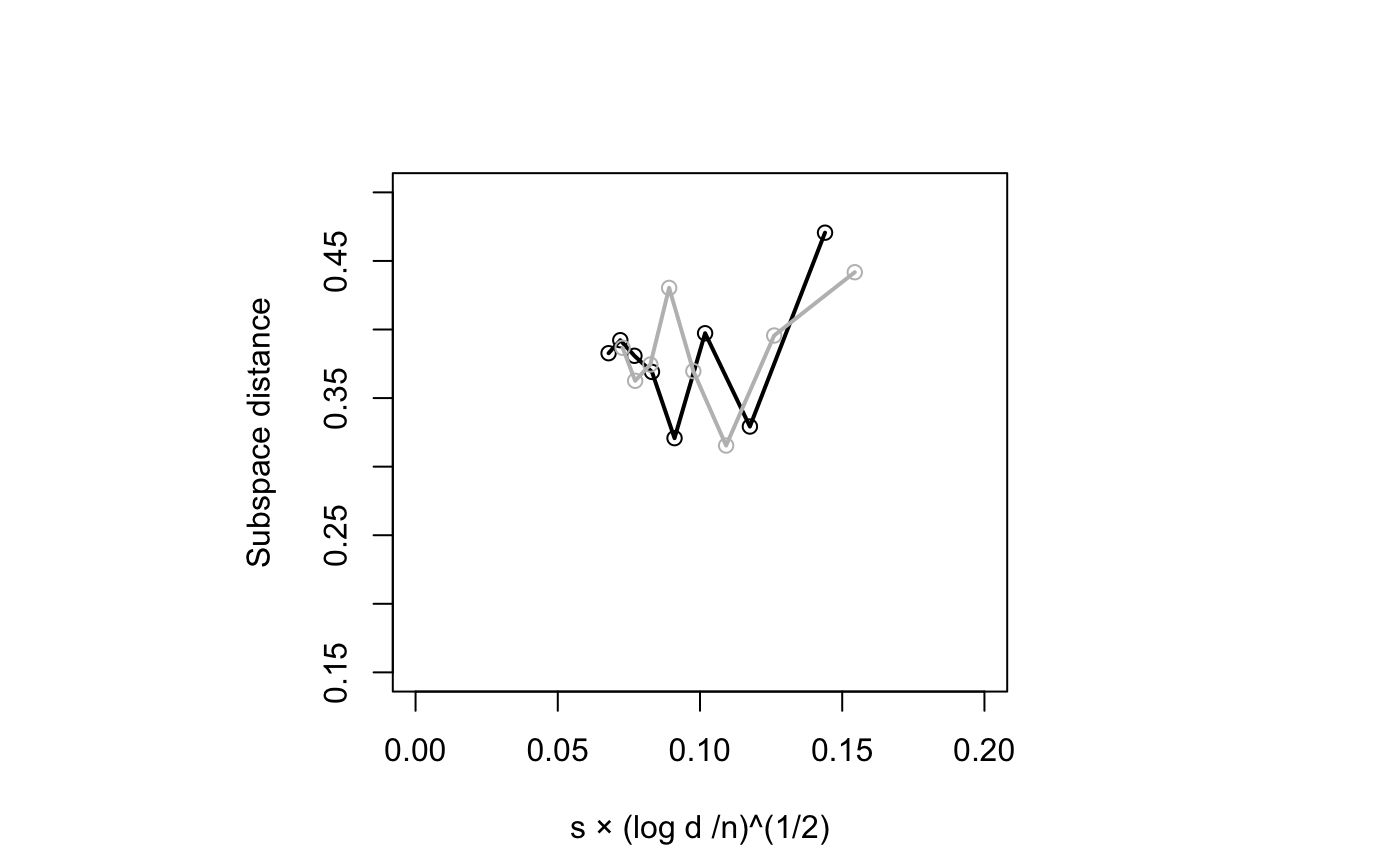
\includegraphics[width=7.5cm]{41.png}} 
\subfigure[Setting 2 case ]{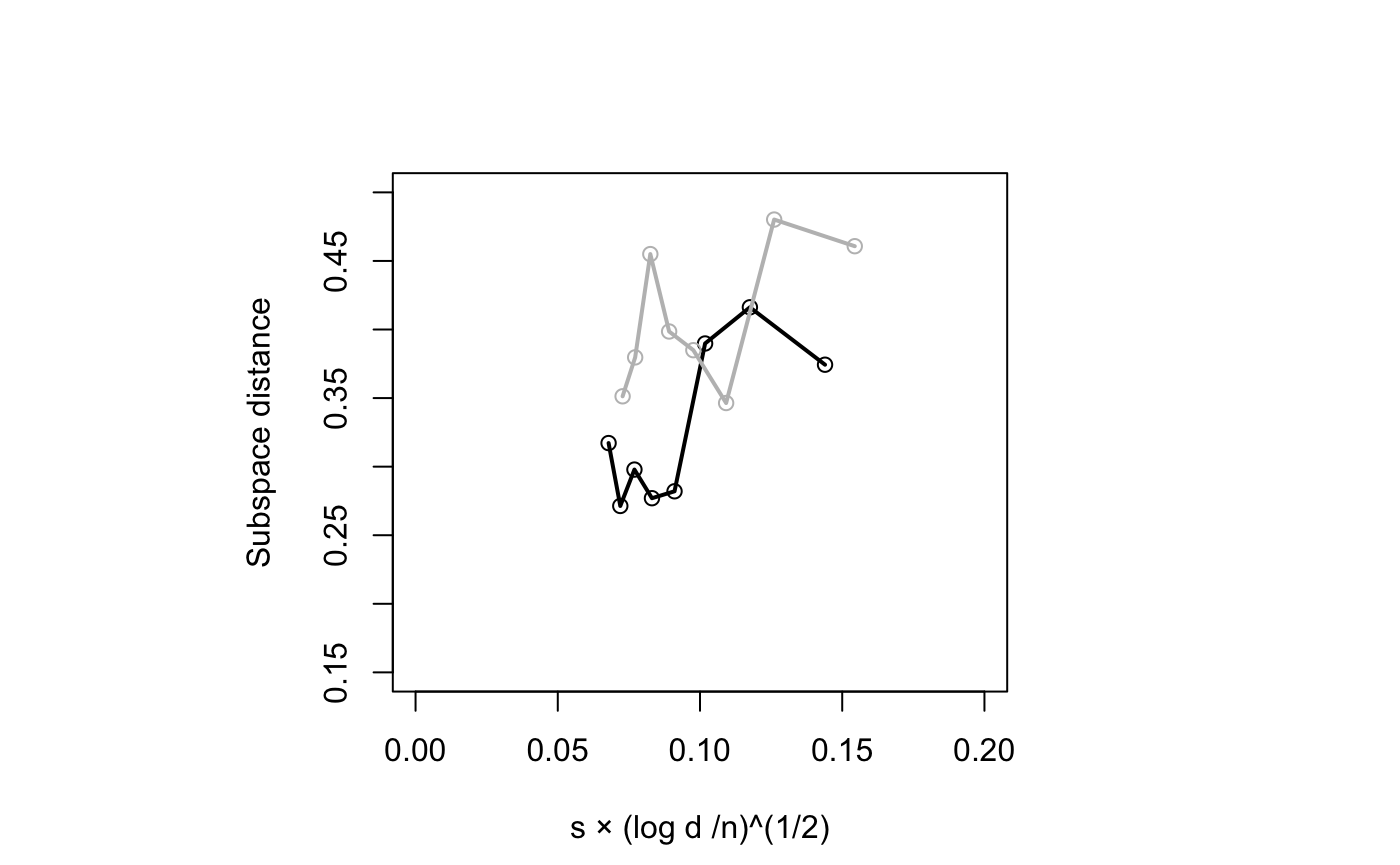
\includegraphics[width=7.5cm]{42.png}}
\caption{ 子空间距离结果,通过改变n得到图中不同的点,其中黑线为d=100,灰线为d=200情形} %图片标题
\end{figure}

\subsection{实验2:论文三个模型下的其他方法比较(实验扩展部分)}

\textbf{\Blue{关于$\lambda$的选择:}} 注意到$\lambda$是我们需要预先选取并通过Cross-Validation 来选取,由于Cross-Validation是非常耗时的,所以预先选取合适的$\lambda $是能有效提升计算速度的。可以看到在各种K下,0.3-0.5之间的阶段的$\lambda$都能达到有一个比较快的迭代速度和稳定性。 而过小或者过大的$\lambda$会导致需要迭代很多次才能收敛或者直接导致给出偏差极大结果。 
\begin{figure}[!htp]
  \centering
  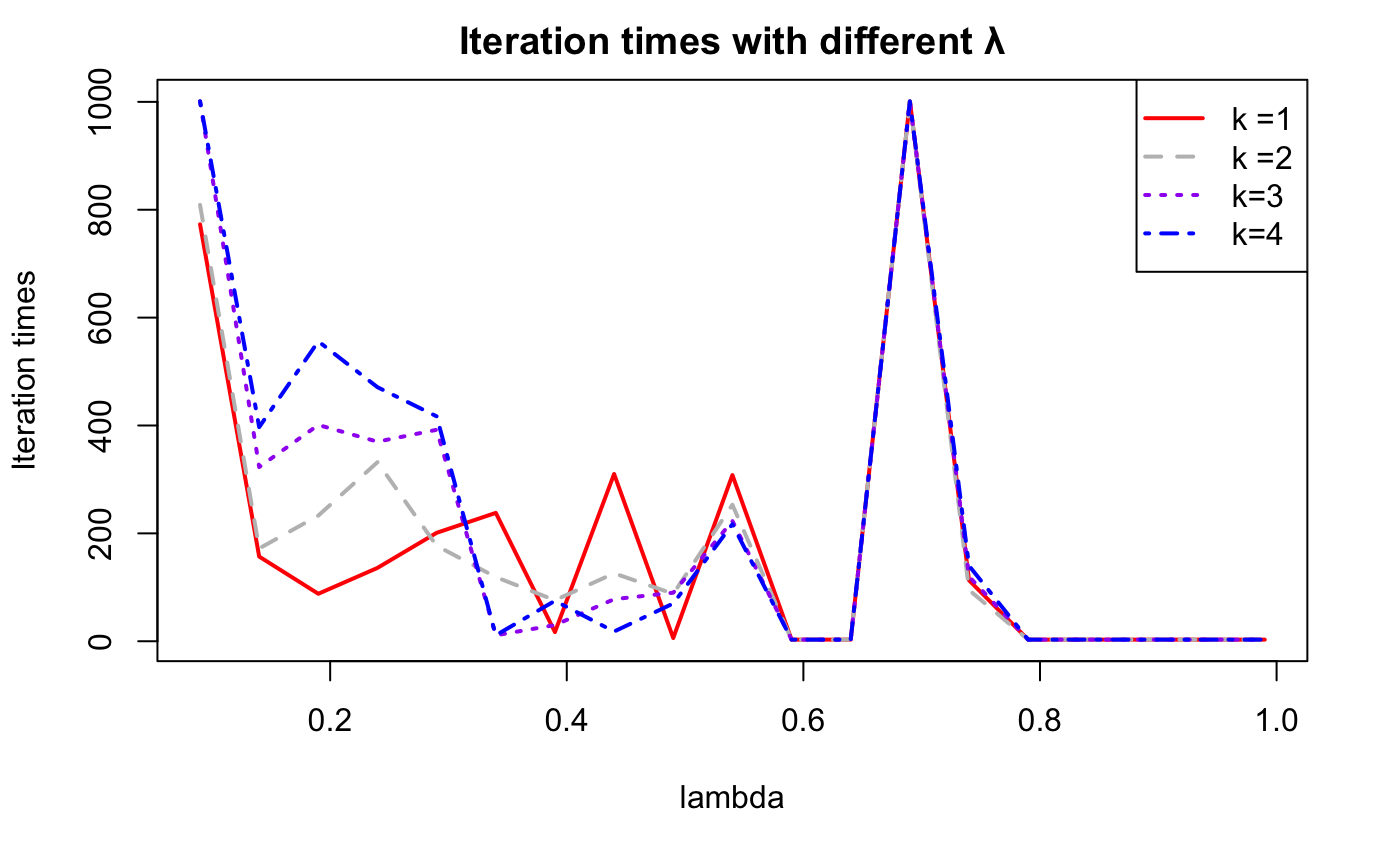
\includegraphics[width=0.72\textwidth]{Select_lambda.png}
  \caption{\small$\lambda $选取与迭代次数的关系}
\end{figure}

\textbf{\Blue{模型1 下的其他算法表现:}} 这里我们使用了Lasso, Ridge and ElasticNet Regression方法在其他设置与 SSIR方法一样的情况下进行对比。其中ElasticNet Regression为一种同时结合$ L_1,L_2$正则化的方法:
$\min _{\theta} \frac{1}{2 m}\left[\sum_{i=1}^{m}\left(\theta^{T} x^{(i)}-y^{(i)}\right)^{2}+\lambda_{1} \sum_{j=1}^{n}\|\theta\|+\lambda_{2} \sum_{j=1}^{n}\|\theta\|_{2}^{2}\right]$

从图2(下一页)可以看出Lasso和ElasticNet Regression都正确的选出了参数,而Ridge则有较大误差。 这与$L_1$正则可产生选择参数效果密切相关。 

\begin{figure}[!h]
\centering
\subfigure[CV Selection]{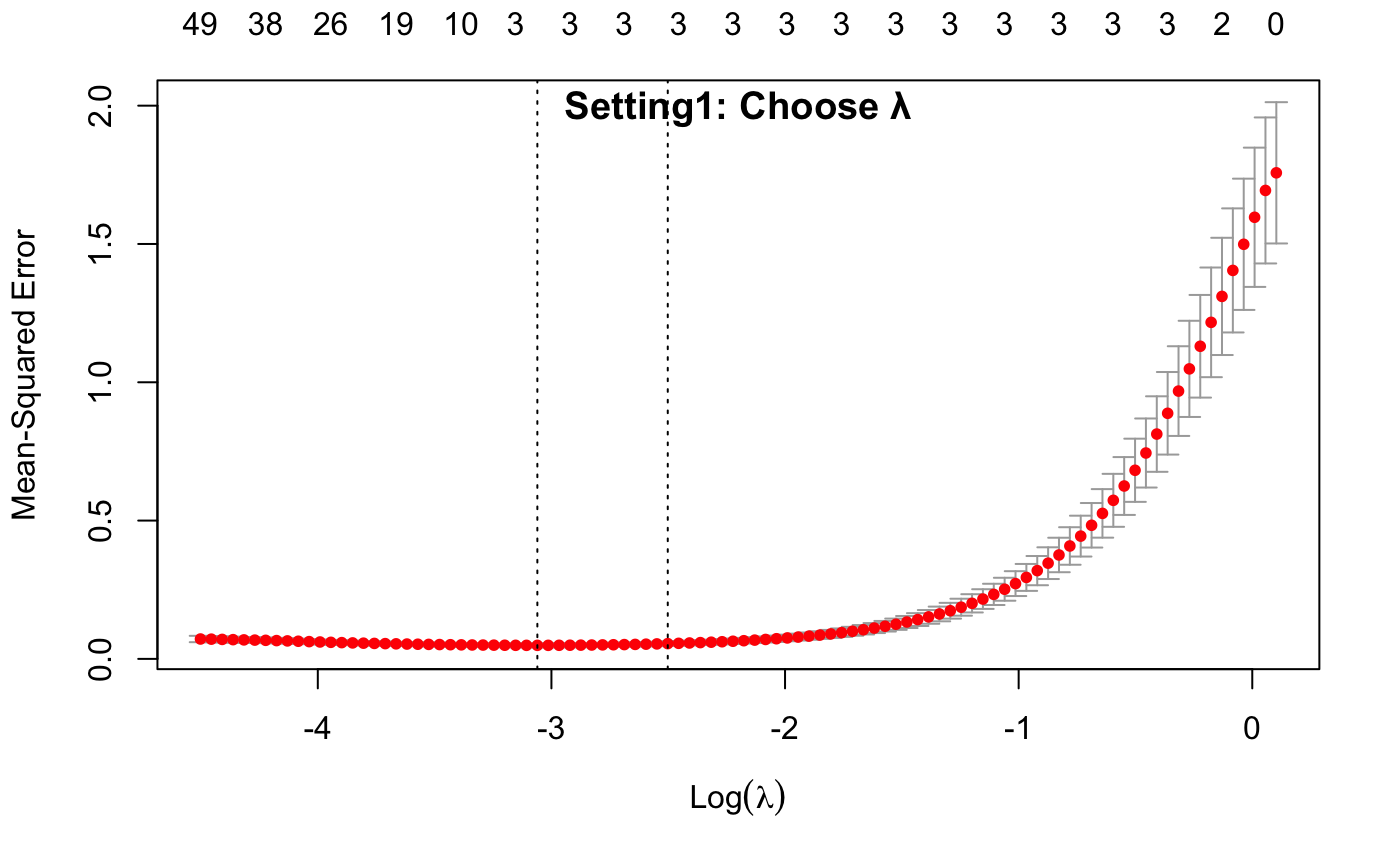
\includegraphics[width=7.7cm]{10.png}} 
\subfigure[Lasso Regression ]{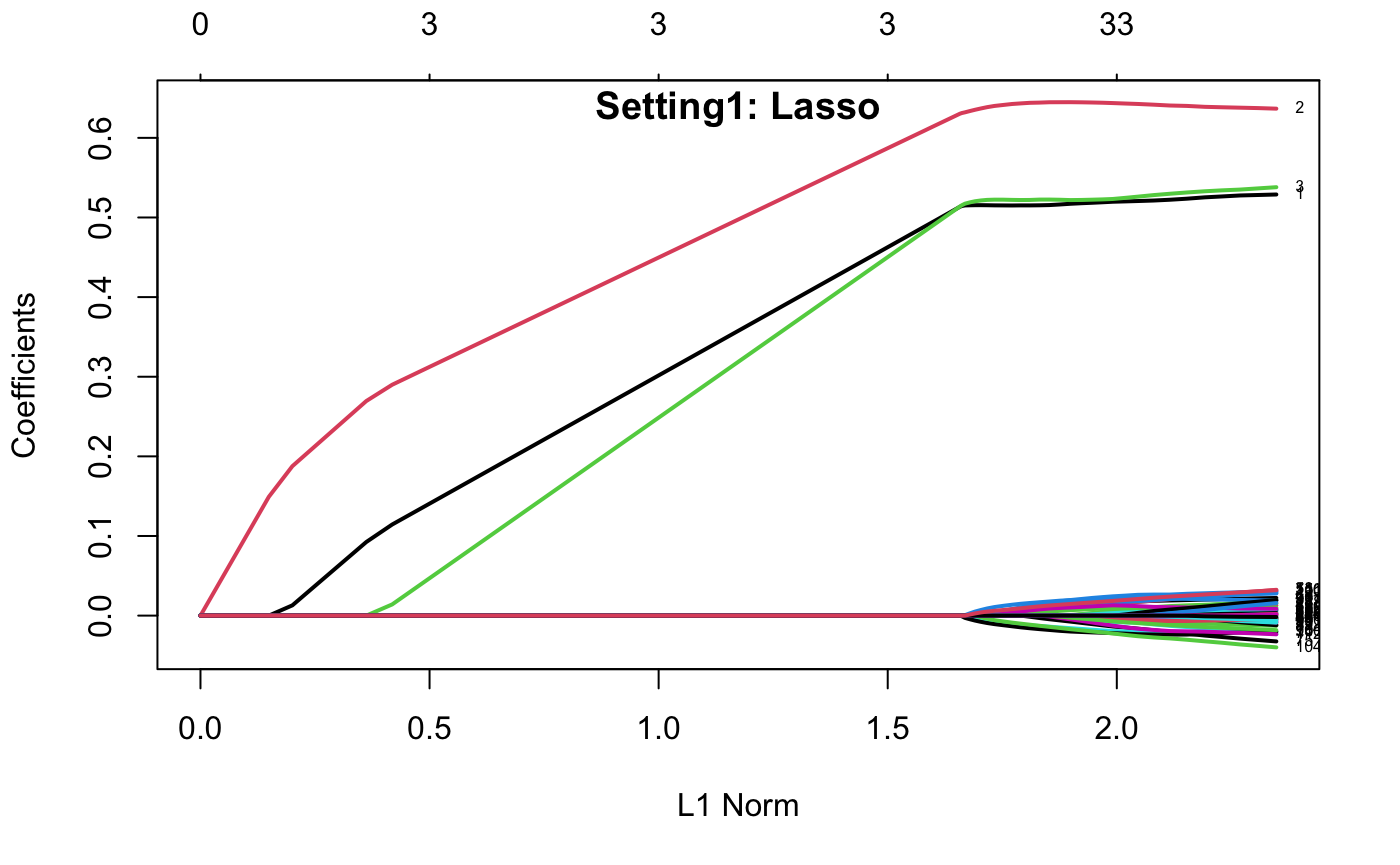
\includegraphics[width=7.7cm]{11.png}}
\\ %换行
\centering
\subfigure[Ridge Regression]{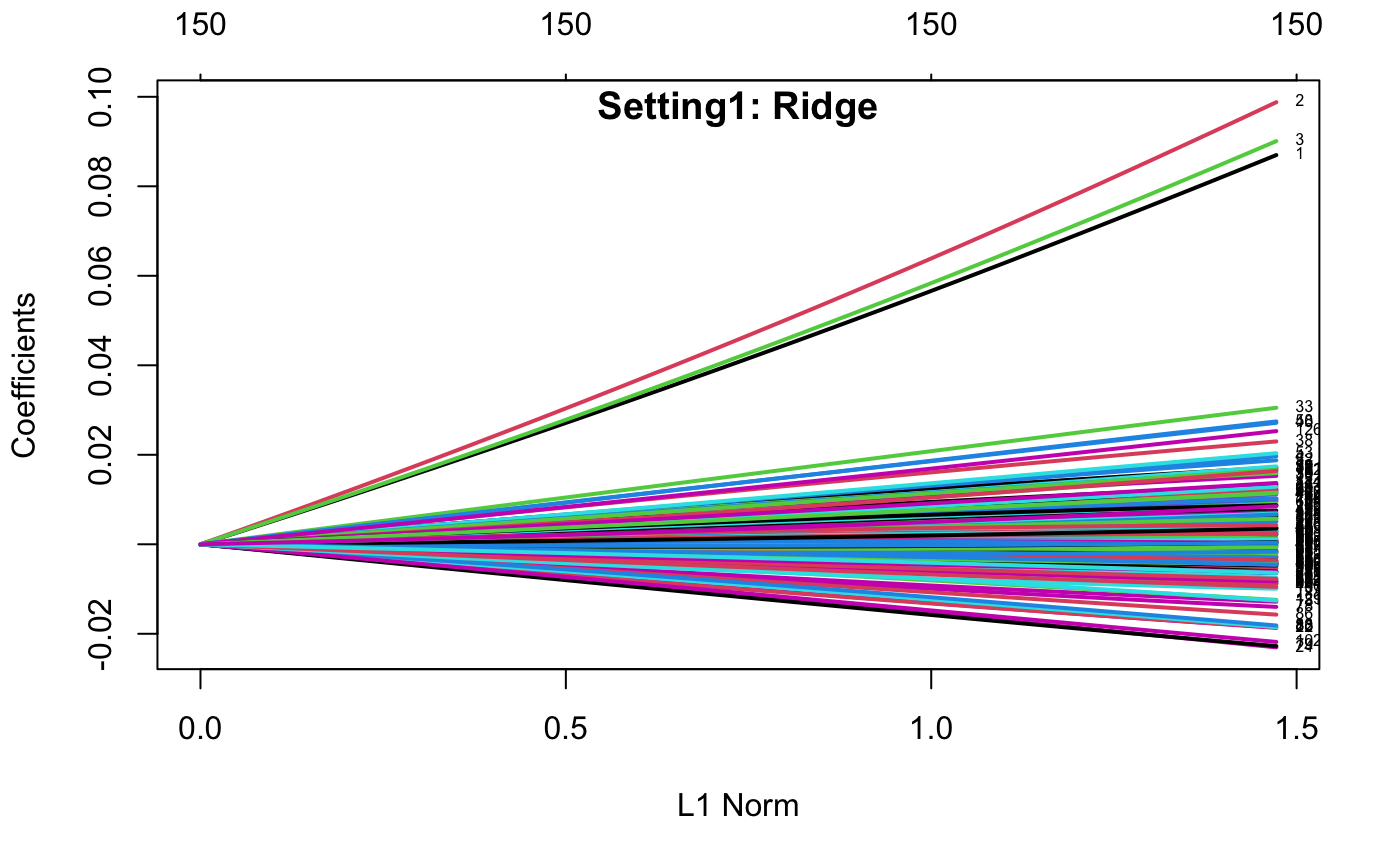
\includegraphics[width=7.7cm]{12.png}}
\subfigure[ElasticNet Regression]{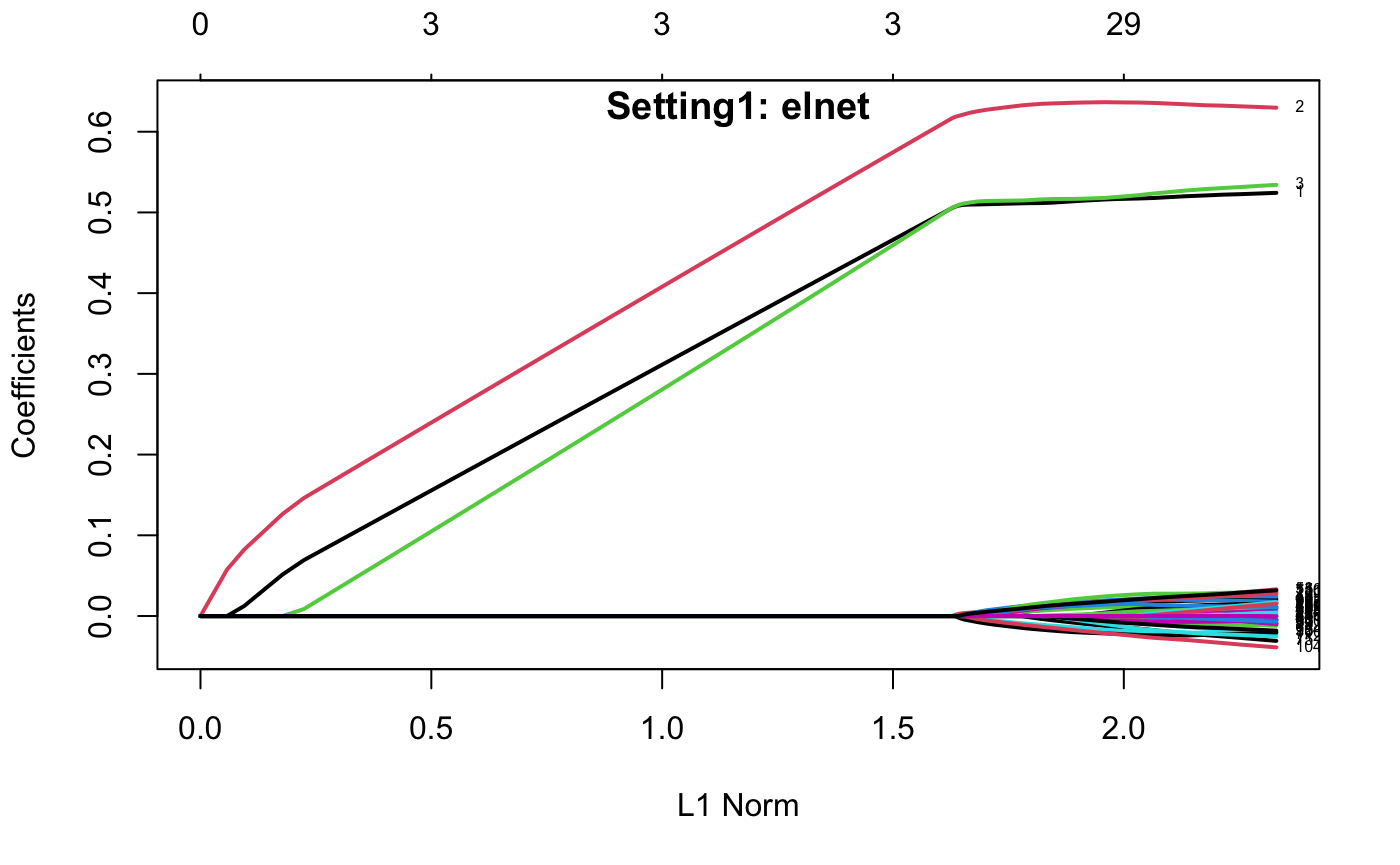
\includegraphics[width=7.7cm]{13.png}}
\caption{Setting 1 下Lasso, Ridge and ElasticNet Regression 的表现} %图片标题
\end{figure}


\textbf{\Blue{模型2和3 下的其他算法表现:}} 由图三(下一页)可以看出在setting 2 和 3的非线性情况下Ridge Regression取得了相对比较好的结果.而Lasso和Elnet表现都不佳。故对于不同模型应选择合适的回归方法,如这三个方法应主要使用于线性模型中。而对于非线性模型,应使用如 SSIR等更加合适的方法。

经实验我们发现,SSIR方法能非常好的在非线性模型下选出显著的变量,即该方法表现受到模型线性/非线性影响较小,适用性广,但其缺点是迭代求解以及要选择合适参数(参数对结果影响很大),计算速度较慢。 所以可在非线性模型情形下在选择使用此法求解得到比较好的结果。
\begin{figure}[!h]
\centering
\subfigure[CV Selection]{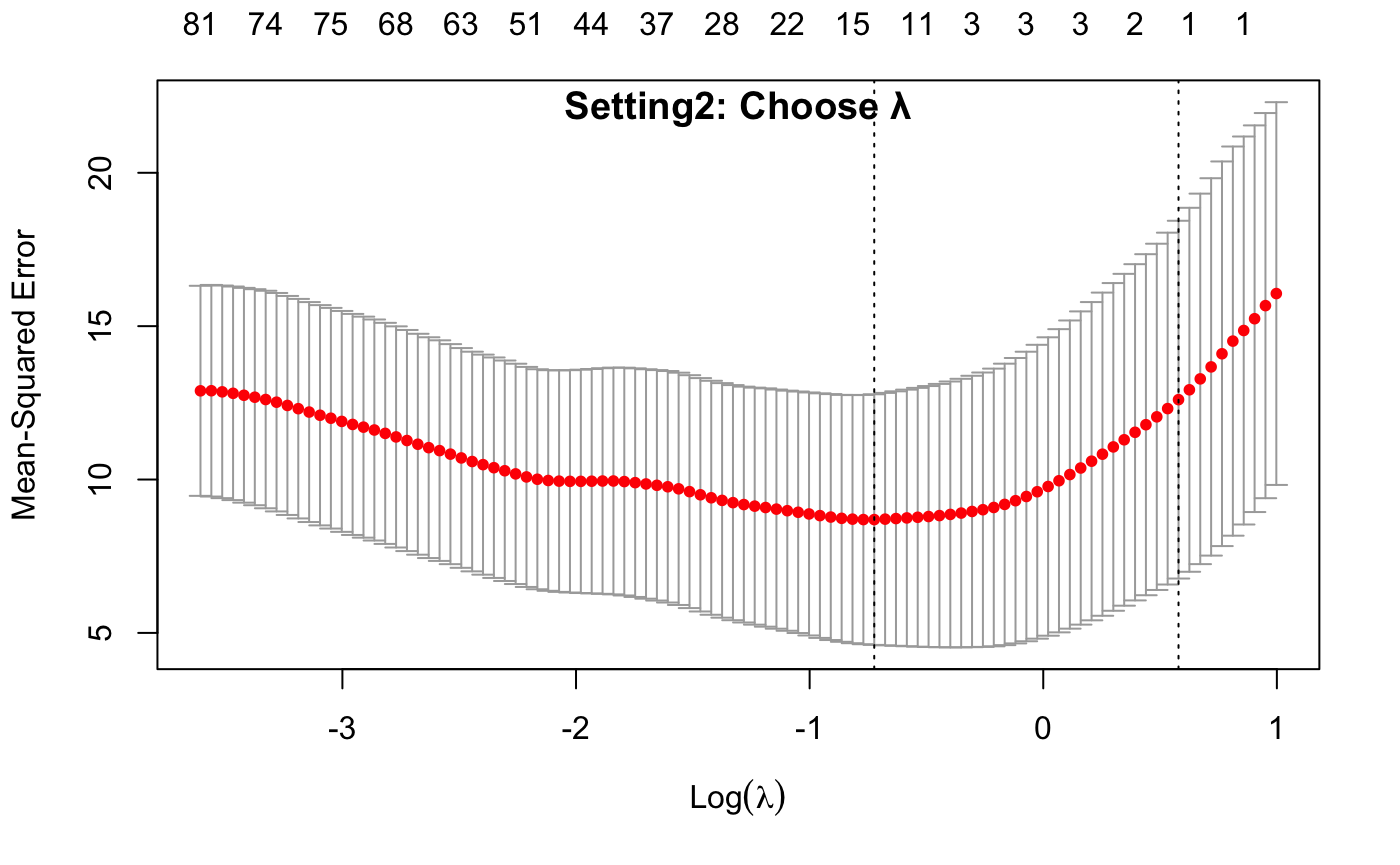
\includegraphics[width=6.5cm]{20.png}} 
\subfigure[Lasso Regression ]{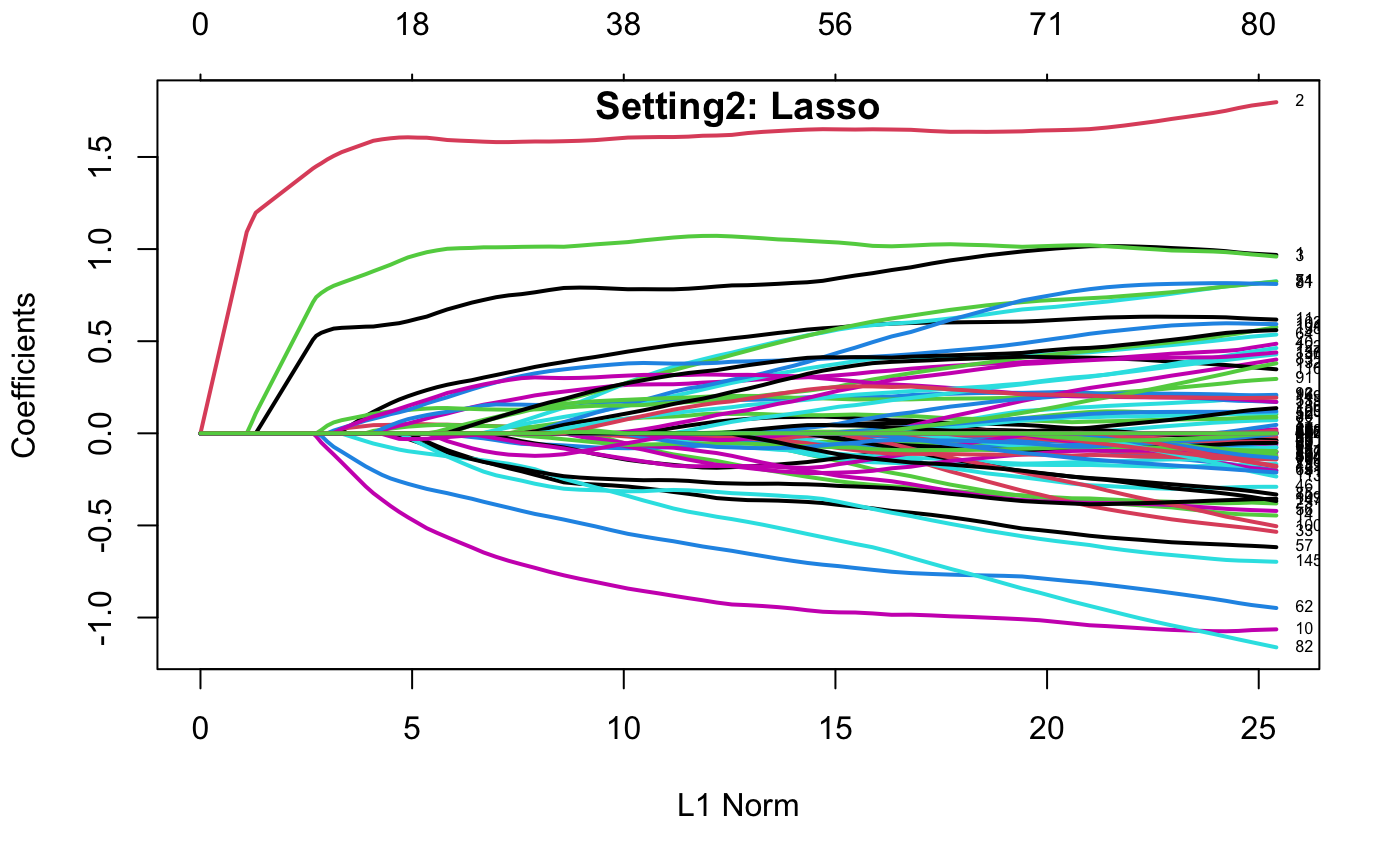
\includegraphics[width=6.5cm]{21.png}}
\\ %换行
\centering
\subfigure[Ridge Regression]{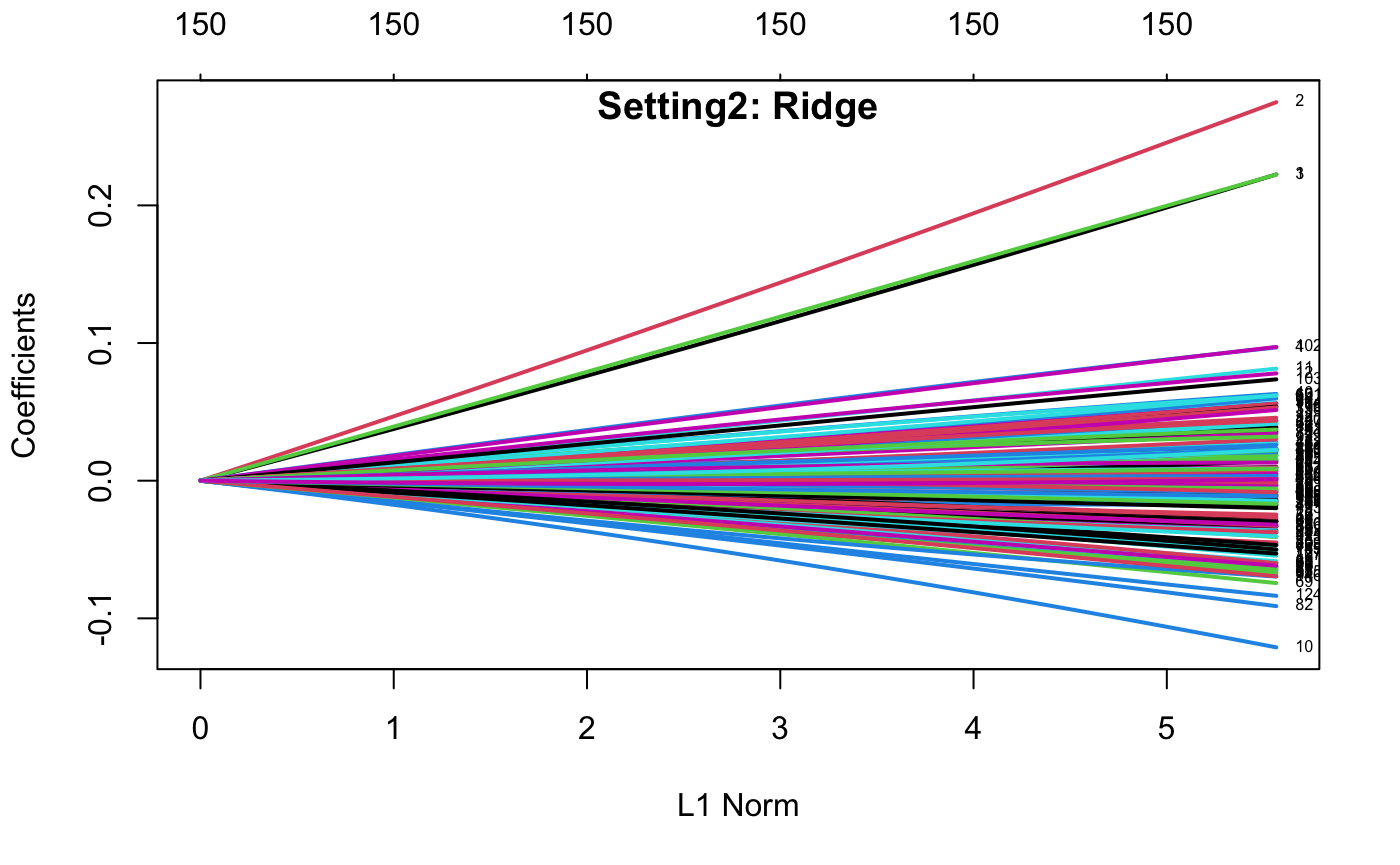
\includegraphics[width=6.5cm]{22.png}}
\subfigure[ElasticNet Regression]{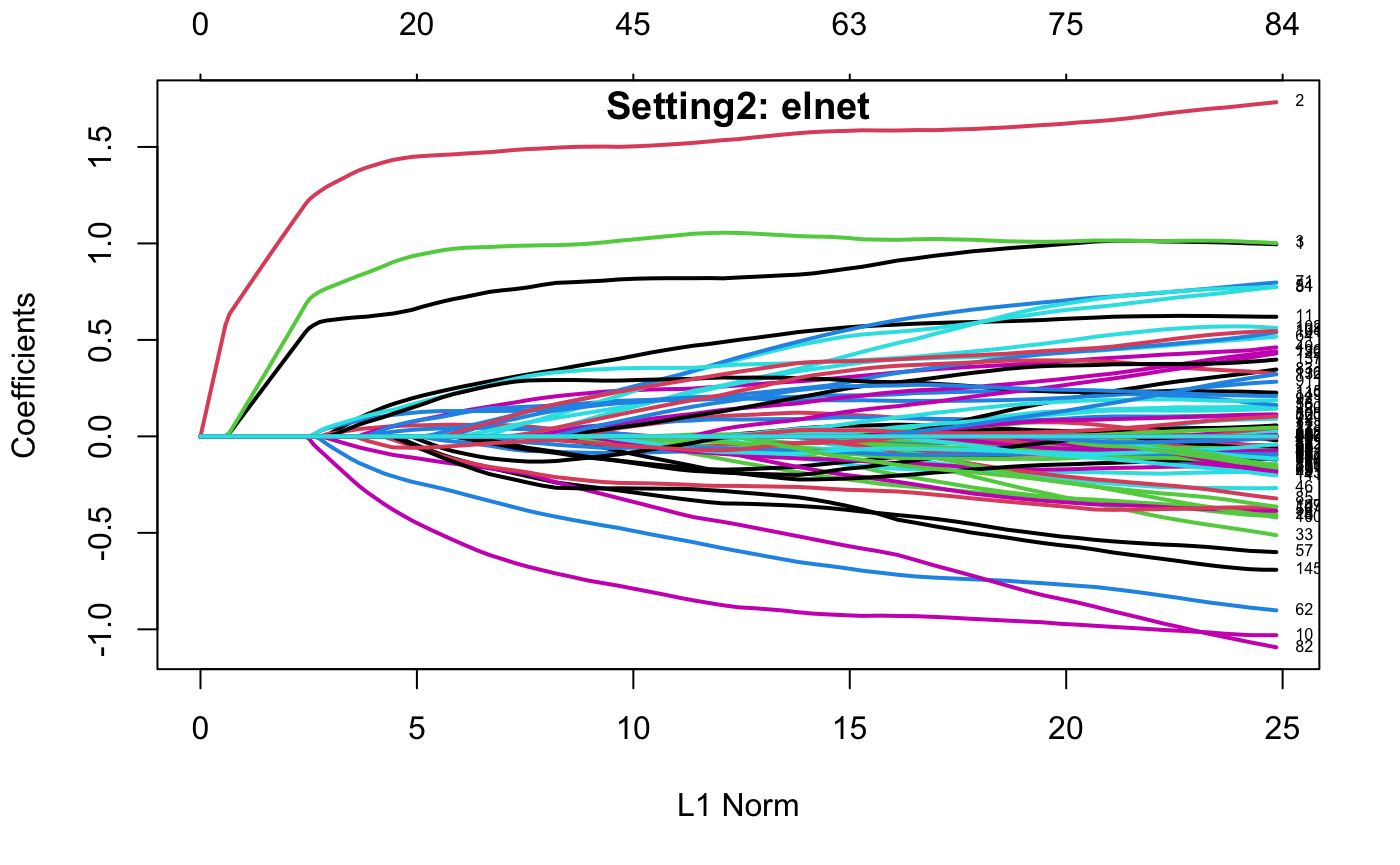
\includegraphics[width=6.5cm]{23.png}}
\caption{Setting 2 下Lasso, Ridge and ElasticNet Regression 的表现} %图片标题
\end{figure}

\begin{figure}[!h]
\centering
\subfigure[CV Selection]{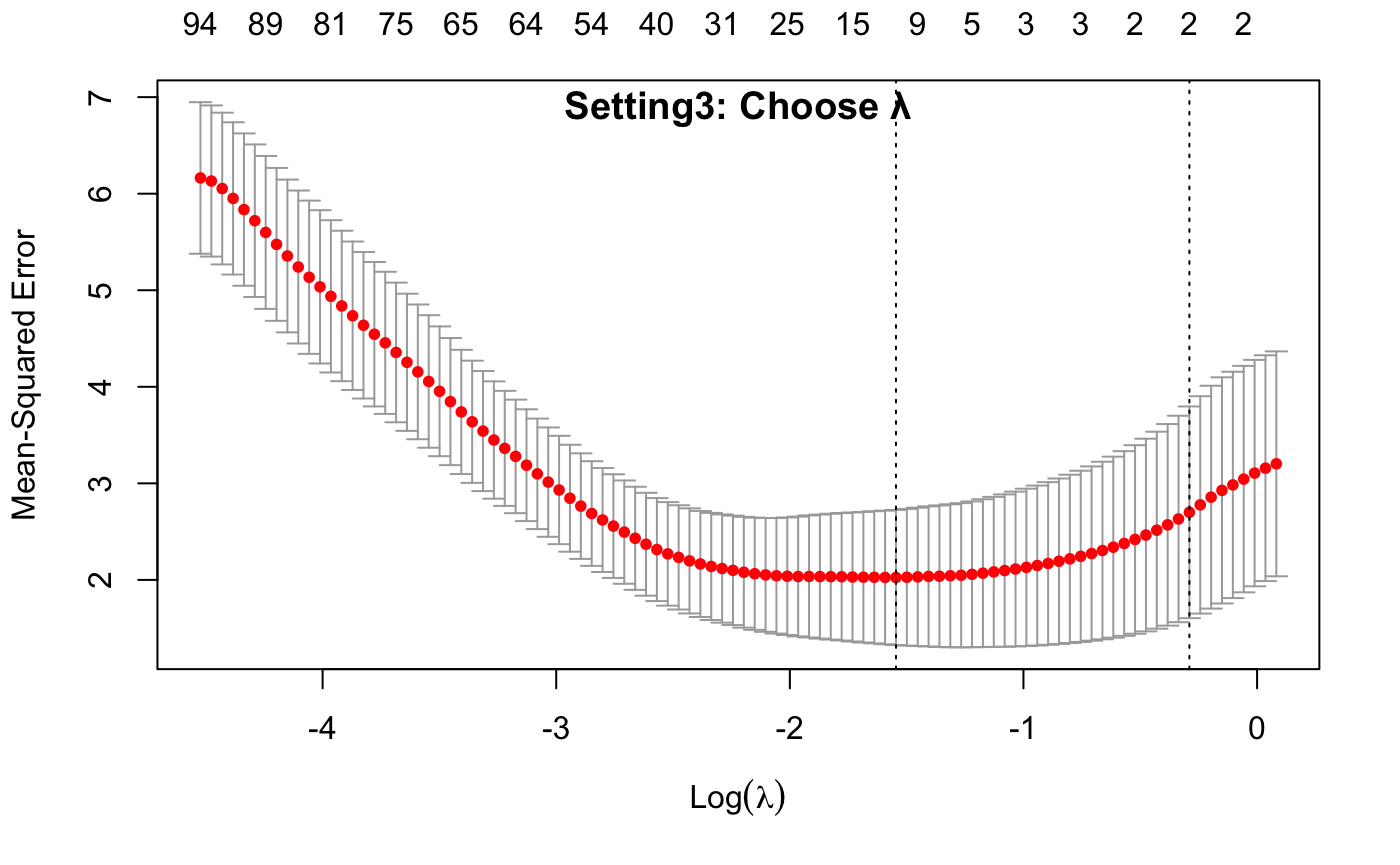
\includegraphics[width=6.5cm]{30.png}} 
\subfigure[Lasso Regression ]{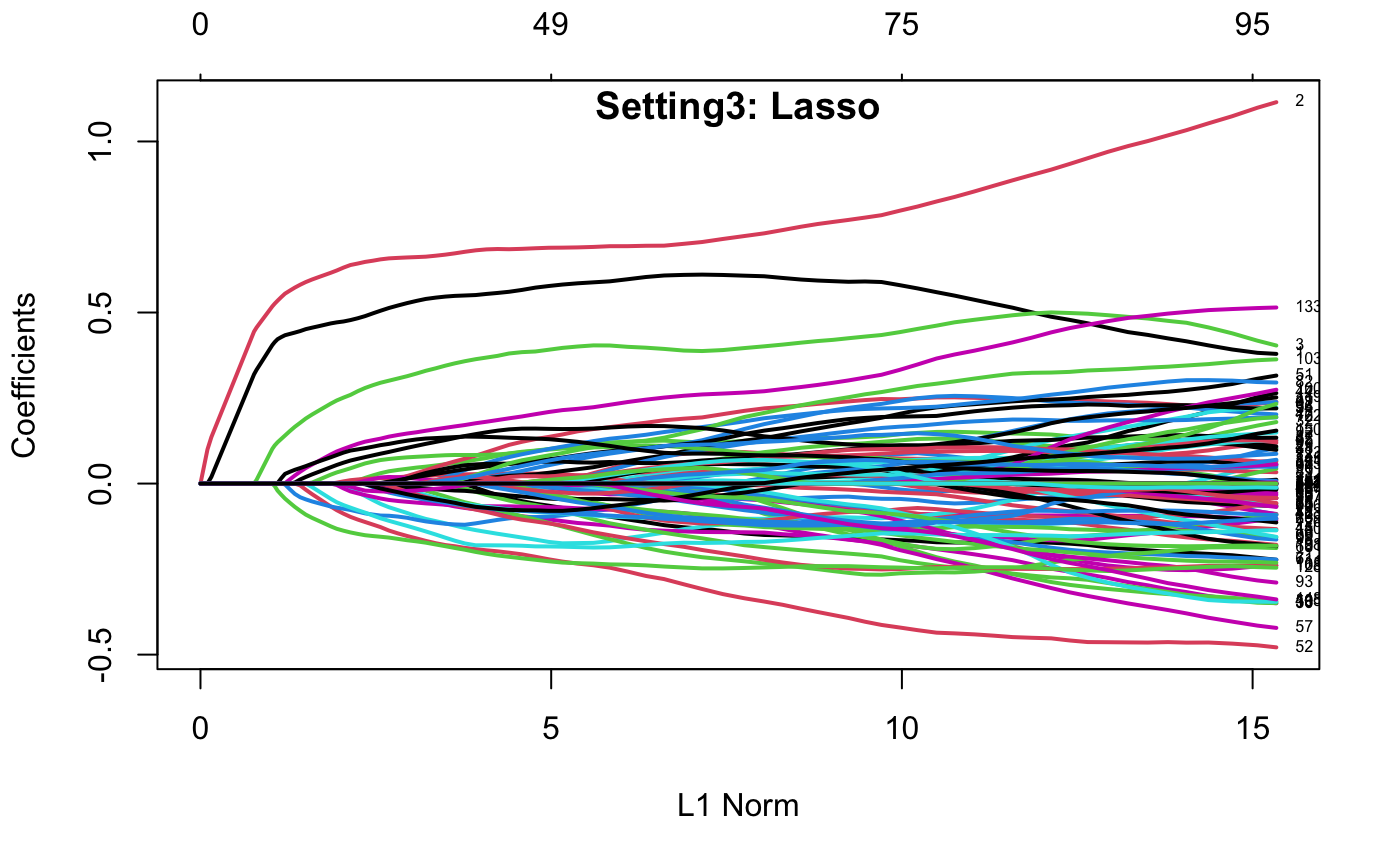
\includegraphics[width=6.5cm]{31.png}}
\\ %换行
\centering
\subfigure[Ridge Regression]{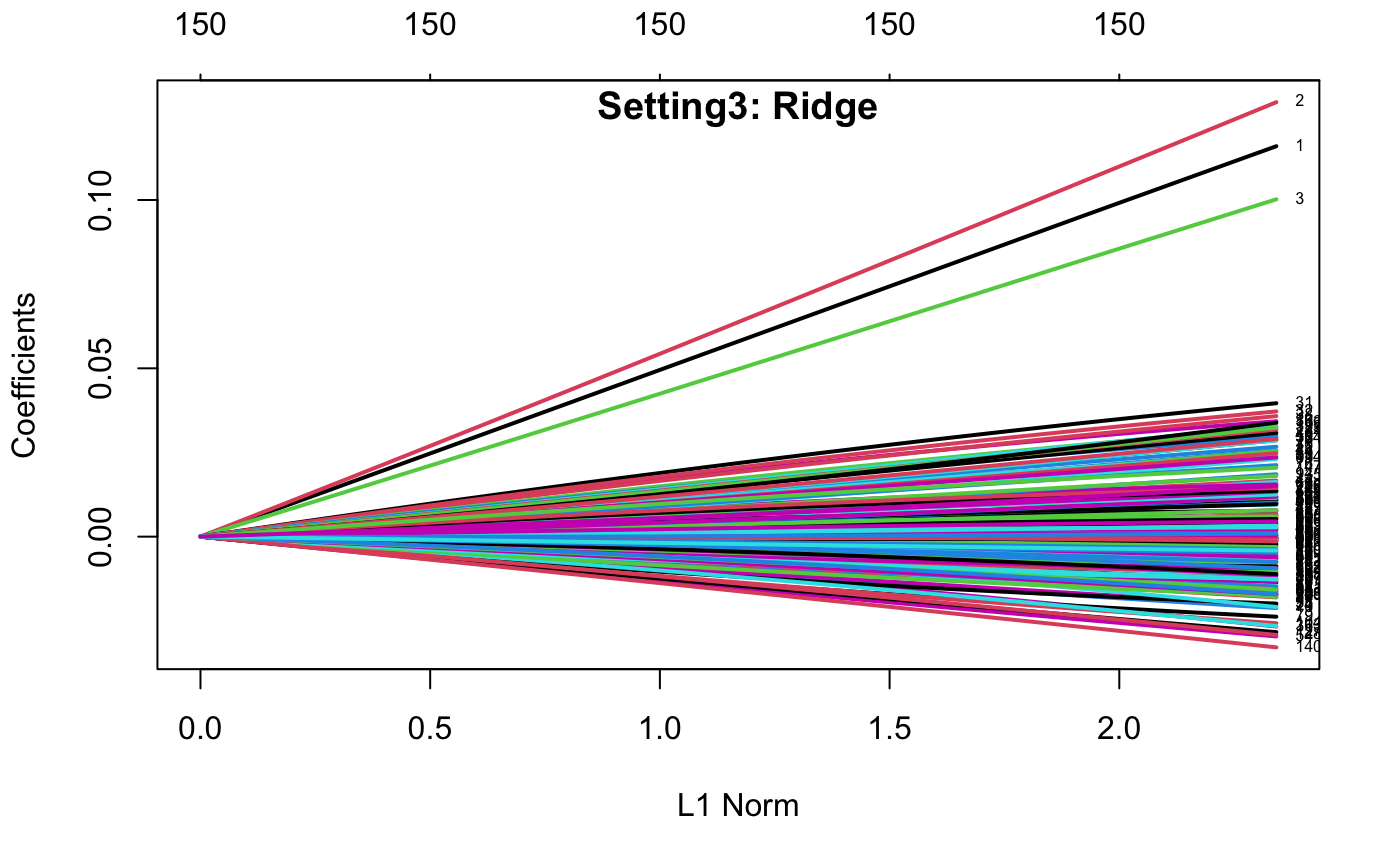
\includegraphics[width=6.5cm]{32.png}}
\subfigure[ElasticNet Regression]{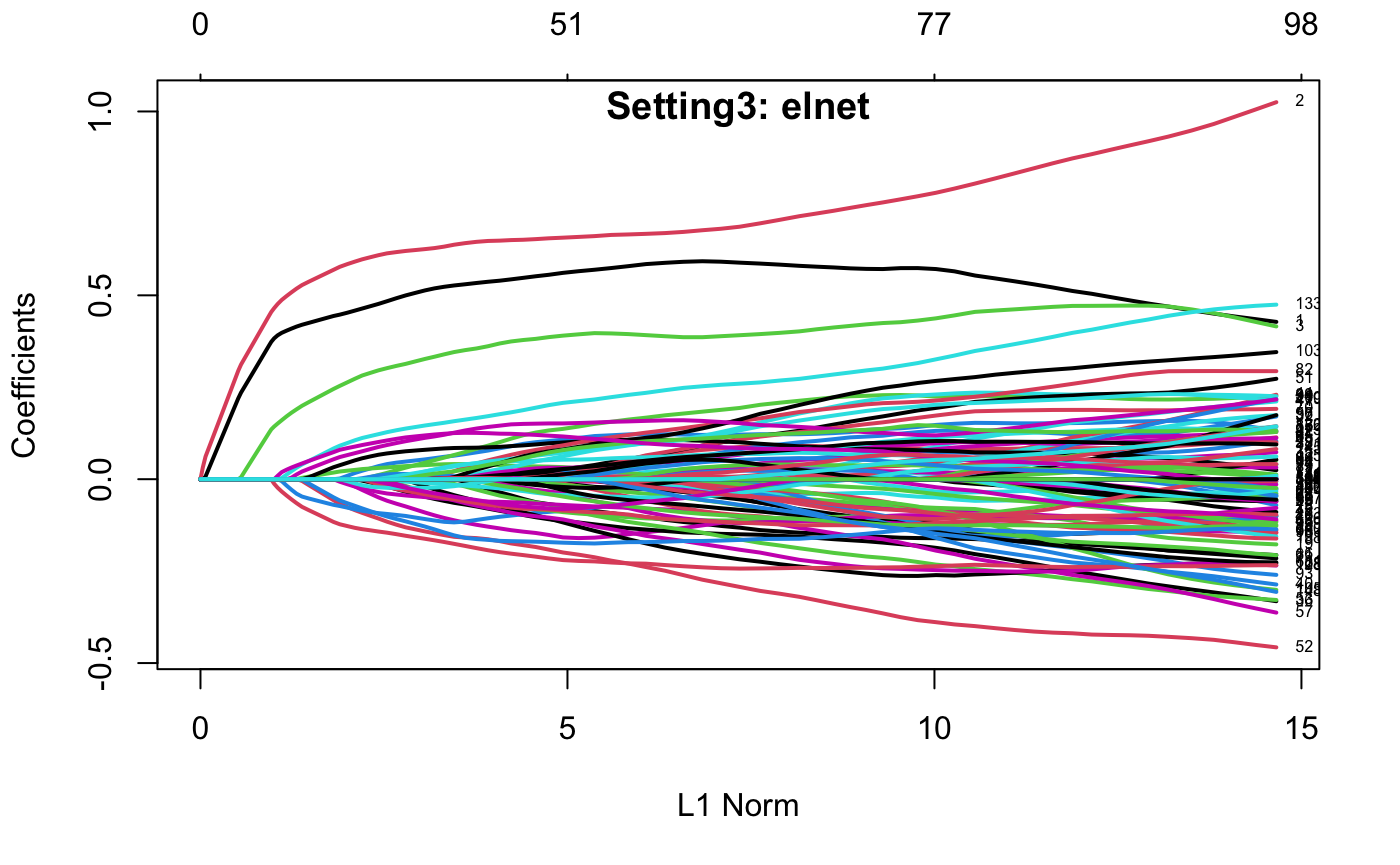
\includegraphics[width=6.5cm]{33.png}}
\caption{Setting 3 下Lasso, Ridge and ElasticNet Regression 的表现} %图片标题
\end{figure}

\newpage

\section{总结与后续讨论}
\large{\textbf{\Blue{项目总结:}}} 
\begin{itemize}
    \item 通过一次完整的阅读和复现过程对整篇文献的理论和实验部分都有了较深刻的理解。
    \item 同时通过复现算法与不断的实验与调试最终得到结果 让我们的理论和代码能力大大提高。 
    \item 最后我们进一步的通过 在模型下实现Lasso,Ridge和Elastic Net回归方法以更深的理解不同方法的优劣和在处理实际问题时 如何选择方法来获得理想的结果。
\end{itemize}


\large{\textbf{\Blue{可以继续优化的地方:}}}
\begin{itemize}
    \item 考虑到cross-validation是计算量的主要来源部分,所以对K值的估计也很大程度影响计算速度和最后的结果。能否有好的方法给出一个K的大致范围是可以考虑的问题。
    \item 方法在更加复杂的模型下是否仍能有比较好的稳定性?以及在更高维度($p>10^4$)的情形下表现如何,都是值得考虑和研究的问题。
\end{itemize}

\subsection{任务分工:} 
\Blue{鉴于各自完成的工作量,我们一致认为两人应平分在这次Project中的贡献。}
\begin{enumerate}
    \item 骆霄龙:  主要负责实验部分以及实验扩展部分代码,撰写项目报告。
    \item 晏若儒:  主要负责复现论文方法,并进行代码优化,展示PPT制作以及Presentation。
\end{enumerate}

\newpage
\nocite{*}
\bibliography{wpref}

\end{document}
